\documentclass[12pt]{article}
 \usepackage[margin=1in]{geometry} 
\usepackage{amsmath,amsthm,amssymb,amsfonts}
  \usepackage{graphicx}
\usepackage{wrapfig} 
\usepackage{color}
\usepackage{verbatim}
\usepackage{multirow}
\usepackage{longtable}
\usepackage{tabu}
\usepackage[utf8]{inputenc}
 \graphicspath{ {Images/} }
 \usepackage{float}
\newcommand{\N}{\mathbb{N}}
\newcommand{\Z}{\mathbb{Z}}
\usepackage{hyperref}
\hypersetup{
    colorlinks=true,
    linkcolor=blue,
    filecolor=magenta,      
    urlcolor=cyan,
}
 
\newenvironment{Project}[2][Project]{\begin{trivlist}
\item[\hskip \labelsep {\bfseries #1}\hskip \labelsep {\bfseries #2.}]}{\end{trivlist}}
%If you want to title your bold things something different just make another thing exactly like this but replace "problem" with the name of the thing you want, like theorem or lemma or whatever
 
\begin{document}
 
%\renewcommand{\qedsymbol}{\filledbox}
%Good resources for looking up how to do stuff:
%Binary operators: http://www.access2science.com/latex/Binary.html
%General help: http://en.wikibooks.org/wiki/LaTeX/Mathematics
%Or just google stuff
\title{Software Engineering\\Project Report}
\author{\textbf{Authors}\\Group 5\\Levi Goldfein 1257360\\Sabeehah Ismail 797621\\ Sergio Oliveira 1101482 \\Storm Menges 1102107}
\maketitle

\begin{center}
\LARGE
\textbf{Shopping Route Recommender\\(SRRec)\\Project 3}
\end{center}
\pagebreak



\tableofcontents
\pagebreak

\section{Project Overview}
The Shopping Route Recommender (SRRec) enables a shopper to map out a route of the nearest shops in the neighbourhood to visit in order to meet their shopping needs. The system will retrieve and display a list of products that are available from the Shops' databases. The shopper/user will select their required products from the list and these will be temporarily stored in a shopping list. When the user has completed their shopping list, the system will search through the database for the relevant stores that sell the selected products. Preference will go to the shops that are close-by and sell all the required products. The system will then use the addresses of these relevant shops to calculate the shortest path, as well as the external tool, Google Maps API, to map out the route and display it to the user.
\\\\
The SRRec has been implemented as a web-application, so that users may access the system on their pc or mobile device (through the web browser). 
Since we have implemented a prototype of the system, we had to make the following assumptions:
\\
\begin{itemize}
\item We are working on a small-world example for now, where there are only a few stores available within the user's vicinity.
\item The starting location is the user's home. 
\item Each shop follows a similar database structure and the same naming conventions.
\item We will not take brands into account, but will use simple product names instead, e.g. bread, milk, eggs, etc. 
\item We do not take stop-overs into account. Stop-overs include coffee, drinks, lunch, etc. 
\item It is assumed that the user requires the route immediately after logging the products in the shopping list. The shopping list is cleared when the user closes the web-application, and will therefore be required to start a new shopping list the next time they request a recommended shopping route.
\item Our system retrieves Product and Price data from Shops that have agreed to give us access to their databases. 
\end{itemize}

\section{Problem Statement}
Our application is setup to address the problem faced by  busy mothers, businessmen and the general population everyday, a lack of time. With the pace of the world increasing all the time,as well as struggling financially, people struggle to go to one shop to purchase their necessities, let alone shop around to get the best bargains and value for money.

\section{Project Objectives}
Our program solves the issues mentioned in the problem statement by taking in a shopping list from the user as input and then searches through our databases for the items requested and then finds the best shops whether by cheapest items or shortest route (requested by the user) and outputs a map with the route of shops the user should take to achieve their goal. Saving them much needed time and money.

\section{Stakeholders and Stakeholder Descriptions}
\subsection{Shopper}
\subsubsection{Goals:}
To receive a recommended route that they can follow in order to find the shops near them, that sell the required items/products that they need to shop for.
\subsubsection{Summary:}
The Shopper is the stakeholder who will make use of our system, the Shopping Route Recommender (SRRec/"the system"). The Shopper (user) will create their shopping list by selecting the products that they need to go shopping for, from a list of products. When the user has completed their shopping list, the system will search for the relevant shops that sell the required products. The system will make use of these shops' addresses to map out the shortest path on the Google Maps API and this route will be displayed to the Shopper to follow
\subsubsection{Environment:}
The SRRec is a web-application and so the Shopper can use the system wherever they have internet
access.
\subsection{Developer}
\subsubsection{Goals:}
To implement a system that recommends a route for the user to follow in order to find shops near them that sell the required items that the shopper requires, in an easy, user-friendly and efficient manner.
\subsubsection{Summary:}
The Developer should analyse, design and implement a web-application that retrieves a list of the
available products from the Shops’ databases. The user must then be able to select their required
products from this list, which will be logged into a shopping list that must be temporarily stored. The
Developer must then implement a function that will search through the Shops in the database for
relevant stores, giving preference to Shops that are close-by and sell all the required products. The
addresses of the relevant Shops must then be parsed to the external tool, Google Maps API, where a
shortest path will be generated, mapped and displayed to the user. The Developer must perform
appropriate testing on the system and functions, as well as perform required system maintenance
and security.
\subsubsection{Environment:}
The Developers workplace.
\subsection{Shop Outlet}
\subsubsection{Goals:}
To gain more customers through this web-application as it recommends the store to Shoppers that
are close-by, granted that the store sells the Shopper’s required items.
\subsubsection{Summary:}
In order for the Shop Outlet to possibly appear on the web-application, the Shop Outlet must give
the Developers access to their database, such as products, prices, and address. This allows the
system to retrieve the list of products available to the user, and use the Shop’s address to generate
the shortest path for the shopping route. It is the responsibility of the Shop Outlet to keep its
database updated and accessible to the Developers.
\subsubsection{Environment:}
The Shop Outlet’s workplace/location.

 \section{System Requirements Specification}
 \subsection{Product Scope} 
Our system is a shopping route recommender (SRRec) that maps out a route of the nearest shops in the user's area. The user will identify the items that they need to go shopping for, which could be groceries, clothing, appliances, etc. The items will be logged into a shopping list. On the user's required shopping day, they will run the SRRec and obtain a recommended route of shops to follow in a particular order to purchase the items they listed.\\\\
The SRRec will be a web-application and therefore should run on any supported web browser that has online access. The database stores each shop in the area with the items that they sell, and their respective prices.\\
Not only will the SRRec recommend a route of shops to purchase the user's required items, but it may also provide a route based on the shortest path for the minimal total expenses or the shortest travel time.\\\\
The benefits of the SRRec are the following:\\
-The user is given a recommended route of the nearest shops in the area to purchase their required items.\\
-If the user wants a route to purchase their items at the cheapest prices, the SRRec will provide a route based on the shortest path for the minimal total expenses.\\
-If the user wants a route that will allow them to purchase their items in the least amount of time, the SRRec will provide a route based on the shortest travel time.

\subsubsection{Purpose}
The purpose of the project is to create quality software that allows 
the user to enter items they require and the software will generate the shortest
path to go and buy the items they require. Our main goal is to produce quality software
that is relevant and provides an accurate solution to all users at any given time

\subsubsection{Product Overview}
Our product is a software product in which we will allow the user to input 
items that they require and we will generate a route which will take the shortest amount
of time, Our product is most likely to target working class people who don't have much time 
to go to the shops. Our product will also include various help buttons and prompts to guide 
users on how to use the software 
\subsubsection{Product Function}
Our product will have one main function which is allowing the user to input 
items that they require and generating a route which will take the shortest amount
of time, we would also like to add a lowest cost route which will take into account 
the petrol spend as well as the prices of the items bought
\subsubsection{User Classes and Characteristics}
Our user class will be a general user with focus
on people who have heavy time constraints with regards to work
\subsubsection{Operating Environment}
The operating environment will be majority of browsers as we will 
integrate support for most big browsers, the coding environment will be Visual Studio and the
Language will be C-Sharp
\subsubsection{Assumptions and Dependencies}
Our assumptions and dependencies include the fact that we will
receive databases of items and their various prices from various supermarkets around Gauteng.
We also assume that all price changes will be updated regularly by the supermarkets and we will 
receive those changes as they happen. To simulate this we will create our own scaled down databases
which will contain a few products and their respective prices


\subsection{Intended User and User Goals}
Our intended user is anyone who needs to go to a store or various stores to do their shopping. The system is aimed to recommend a shopping route for the user to follow, based on the items they require. This route could be the shortest path for the minimal total expenses or the shortest travel time to purchase all the items.
\subsubsection{Key High Level Goals and Problems}
The user may not know where to go in order to purchase all the items they need. The user may also require a route that allows them to buy the items at the cheapest prices, or a route that takes the least amount of time.
With this system, not only will the user be given a recommended route to shop for their items but it may also provide a route for minimal expenses or shortest travel time.
\subsubsection{User Level Goals}
To enter the items that they need to go shopping for and thereafter obtain a recommended shopping route to purchase these items for the minimal total expenses or the shortest travel time.
\subsubsection{Environment}
Either at home, work, or anywhere with online access.

\subsection{Constraints}
\subsubsection{Legal Issues}
We may come across issues where shops may not want to share their databases (such as items and prices) with us. Therefore, if we populate our system's database with such information, we may incur legal ramifications due to breach of confidentiality and incorrect listings of data. 
\subsubsection{Implementation and Software}
If we do come across issues whereby we cannot use a shop's database, our system may not make use of it in the Path Finding Algorithm and therefore the shop won't be listed on the route. This could lead to a situation where the shop may be in the shortest path but because we cannot make use of it, the user may not obtain an accurate route based on their surroundings or shopping requirements.\\\\
We are limited by our implementation time as we are students with our own time constraints.\\\\
Since we plan to make use of Google Maps API for mapping the shopping routes, we are limited to the stores that exist on Google Maps.\\\\
Our system's database is limited to the regular pricing of items as we do not take into account item sales that can occur at shops. This also leads to a situation where our system generates a path that may not be accurate according to real-time changes.\\\\
The user is constrained to using a supported browser in order to make use of our web-application.
\subsubsection{Hardware}
Since our system is an online web-application, it is constrained by the response time and performance of the server and internet connection.

\subsection{Pricing and Implementation Costs}
The possible costs that we may incur are:\\\\
-A domain for the web-application.\\
 R197 once-off   (.co.za)\\
 https://www.afrihost.com/site/product/domain{\_}registration\\\\
-A server to host the web-application.\\
R4850(\$358) upfront \\
(Standard 1 year term: t2.micro for Windows with SQL Web in EU-frankfurt)\\
https://aws.amazon.com/ec2/pricing/reserved-instances/pricing/\\\\
-Development time and maintenance.\\
Subject to working hours and consulting rates of the development team.

\subsection{Quality}
\subsubsection{Correctness}
The user will create an account if they are not registered on the system. If the user has an account then they will log in. The user then enters the items they require and will run the SRRec when they want to go shopping.\\
When the user runs the software, the SRRec must take the user's list of items, compare it to the system's database, run the required Path Finding Algorithm (shortest path for the minimal total expenses or the shortest travel time) and return the mapped-out route to the user.
\subsubsection{Reliability and Efficiency}
Because the SRRec is a web-application, the reliability of the system is reliant on the performance and response time of the server and internet connection. 
\subsubsection{Integrity}
Since the SRRec generates the required shortest paths by making use of the data from various shops' databases, we need to ensure that these databases are secure to protect each store's confidentiality. \\
We should make use of SSL, TSL, and HTTPS to ensure security within our system's online connections and data communications.
\subsubsection{Usability and Portability}
Since we do not plan on including a help function (for novice users) within our web-application, we want to implement the user interface to be as simple and user friendly as we can make it, to promote ease-of-use over ease-of-learning.\\
We will make use of HCI principles and keep consistency throughout the web-application's interfaces. This will allow users to become comfortable and familiar with using the system.\\
Since the SRRec is a online web-application, it can be used on all supporting web browsers (PC and mobile devices) and this allows the user to run the SRRec wherever they may be, granted they have good internet connection.\\
\subsubsection{Maintainability, Flexibility and Re-usability}
Throughout implementation, we will develop the back-end and front-end software in a logical and consistent way so that we may easily make software changes if needed and if a problem occurs, we may locate and fix the issue easily. This also allows us to adequately reuse some parts of the software.
\subsubsection{Testability}
To ensure that our system is implemented correctly, we will make use of interface, validation and database testing.\\\\
Interface testing will be used to check that all UI components (such as buttons) work and trigger their respective processes such as passing data from the forms to the database, changing pages, etc.\\\\
Validation testing will be used to check and ensure that all data entered and passed from the interface forms to the database is of correct data type and format.\\\\
Database testing will be used to check and ensure that data is captured and stored correctly within their respective data stores and attributes. This also ensures that our Path Finding algorithm retrieves and makes use of correct data to provide an accurate route to the user.\\\\
Algorithm testing will be used to check and ensure that our Path Finding algorithm works and produces a correct route that is also mapped-out for the user.


\subsection{External Interface Requirements}
\subsubsection{User Interfaces}
The design of our user interface plans to include both elegance and functionality, the GUI design is planned to suit all users and allow for users of all ages to easily engage with the application. We plan to ensure that our application has ease of navigation and a user interface that is both stylish and current.
\subsubsection{Hardware Interfaces}
Due to the sheet scale of the project the need for dedicated devices and support hardware is not necessary at this point in time, but as the project start to gain popularity amongst users it could call for the use of large scale severs to sore all user information, that would need to be based around the world to ensure that all users from all corners of the globe get the same quality software.
\subsubsection{Software Interfaces}
Our software plans to make use of MVC( Model-View-Controller) architectural pattern which separates an application into three main components:\\
-	Models : Models objects are the part of the application that implement the logic for the applications data domain, they often retrieve and store model state in a database.\\
-	Views: Views are the components that display the applications user interface \\
-	Controllers: Controllers are the components that handle user interaction, work with the model , and ultimately select a view to render that display. The controller handles and responds to user input and interaction.\\
   

Our database will be developed on a SQL server as it works well with the MVC framework as well as C-Sharp, has a huge amount of functionality and allows for scalability and growth of the software if needed. 

\subsection{System Features}
\subsubsection{Minimum Shopping Expenses 1}
\subsubsection*{Description and Priority}
Priority: Very High\\
 The user inputs their shopping list of, say n, items the program then outputs a list of n or less (if 2 or more items are available at the same shop) shops that supply the items on the shopping list for the cheapest amount possible. The output will also show which shopping list items can be purchased at which shop. This feature gives the user no indication the order in which listed shops should be visited.  
 \subsubsection*{Stimulus and Response Sequence}     
-User types in shopping list\\
-User presses button labelled "Shopping Route Recommender?"\\
-System outputs table of shops and products\\
 \subsubsection*{Functional Requirements}
 The requirements for this feature are a database  containing shops (for example: PNP,Checkers,game, DionWired, Mr Price, Woolworth) that stock items an average shopper may need, for example: clothing, groceries, appliances etc, and specific items stocked in said shops with their respective prices. The product should also respond to invalid inputs and errors with an error message. Invalid inputs include items entered that are not found in the database.
 
 \subsubsection{Minimum Shopping Expenses 2}
\subsubsection*{Description and Priority}
 Priority: High\\
 This feature is basically an extension of Minimum Shopping Expenses 1 (feature 2.1), but incorporates the vital goal of the product: a route to take. The user inputs their shopping list of, n, items and their current location. The program then outputs an \textbf{ordered list} of n or less shops to visit and which items are available to purchase at each shop. The shops listed are to provide the user the cheapest possible shopping expenses and are ordered to provide the shortest route while minimum price is prioritised. The route length is irrelevant. 
\\\\
\textbf{Map:} A further extension of this feature will be to show the shops on a map with directions of the route.
 \subsubsection*{Stimulus and Response Sequence}
-User types in shopping list\\
-User presses button labelled "?Shopping Route Recommender?"\\
-System outputs table of shops and products\\
-System outputs map with directions\\
 \subsubsection*{Functional Requirements}
 The basic requirements are the same as Minimum Shopping Expenses 1 with the added information of each shops GPS co-ordinates. As well as the added software capabilities of resolving precise locations and mapping.
 
 \subsubsection{Minimum Travel Time}
\subsubsection*{Description and Priority}
 Priority: High\\
 This feature uses the same input information as Minimum Shopping Expenses 2 (feature 2.2) (shopping list and current location) and outputs an ordered list of shops with preference to a short route length and travel time over actual shopping expenses.  
\\\\
\textbf{Map:} A further extension of this feature will be to show the shops on a map with directions of the route.
 \subsubsection*{Stimulus and Response Sequence}
-User types in shopping list\\
-User presses button labelled "?Shopping Route Recommender?"\\
-System outputs table of shops and products\\
-System outputs map with directions\\ 
\subsubsection*{Functional Requirements}
Will require software to calculate shortest route and perhaps traffic awareness and avoidance  protocols.
 
 \subsubsection{Minimum Total Expenses}
\subsubsection*{Description and Priority}
 Priority: High\\
 This feature requires the same input as features 2.2 and 2.3 and outputs an ordered list of shops that takes into account both shopping expenses and travelling time and expenses and minimises both. 
 \\\\
\textbf{Map:} A further extension of this feature will be to show the shops on a map with directions of the route.
 \subsubsection*{Stimulus and Response Sequence}
 -User types in shopping list\\
-User presses button labelled "?Shopping Route Recommender?"\\
-System outputs table of shops and products\\
-System outputs map with directions\\
 \subsubsection*{Functional Requirements}
 This feature requires up-to-date information on travelling expenses (from the AAA or the likes).
 As well as the functional requirements listed in Features 2.2 and 2.3.
 %new lines to put Section 2.5 to the next page
 \\
 \subsubsection{Account/Login}
\subsubsection*{Description and Priority}
 Priority: Medium\\
 This feature will enable users to sign-up and create an account which enables them to store pertinent information, such as:\begin{itemize}
  \item favourite shopping list
  \item favourite route or route type e.g.: Minimum Shopping Expenses
  \item home/work/starting location
\end{itemize}
for future use. \\
The inputs for this feature would be a valid user-name and password and some form of verification e.g.: email address or cellphone number. 
      
 \subsubsection*{Stimulus and Response Sequence}
-User enters Sign-Up page to create an account \\
-System creates the necessary databases for the user\\
-User enters preferred information e.g.: favourite shopping list\\
-System saves information in correct tables in database
 \subsubsection*{Functional Requirements}
The requirements for this feature would extend to added databases to store user-name password keys,  saved shopping lists and routes and saved locations. We would also have to provide security to ensure none of the users sensitive data is accessible. 

 \subsubsection{Item Success Tracking}
\subsubsection*{Description and Priority}
 Priority:Low\\
 This feature would be an add-on to all the above route features and would remind you which items to purchase at the current shop and then track the success of your stop at the specific shop. This would enable you to recalculate your current route based on whether you found the item at this shop or not. As well as notify other users of the availability of an item at a specific shop.  
 \subsubsection*{Stimulus and Response Sequence}
-When the user arrives at a shop the system outputs which items off  the users shopping list are intended to purchased at this shop.\\
-User  inputs whether or not they were successful.
 \subsubsection*{Functional Requirements}
 This feature would require constant access to the users GPS and perhaps some added input from the user.
 
 \subsection{Security Requirements}
 This product has several security and privacy issues that must be addressed. Concerning user authentication the product will require a valid email address to create an account, then they will require a unique user-name and password pair to ensure no cross contamination of private user information and to prevent access to the users sensitive and personal stored information, such as home or work address, email address, password and frequent or favourite routes. The developers will also have to provide guarantees to participating shops that provide classified and valuable databases of their stock prices that no malicious user or third party will be able to obtain this data beyond the intended scope of the product. 

\section{Use Case Set and Descriptions}
\begin{tabu} to \textwidth{| X[c] | X[c] | X[c] |} \hline
\textbf{Use Case}&\textbf{Description}&\textbf{Actors}\\ 
\hline
Create Shop & This use case creates a new Shop in the shop datastore,in the system's database & Developer\\ 
\hline
Read Shop & This use case allows the user to search/view a Shop from the Shop datastore, in the system's database & Developer\\ 
\hline
Update Shop & This use case updates
details/attribute values of a Shop from the Shop datastore, in the system's database. & Developer , Shop outlet (external)\\
\hline
Delete Shop & This use case deletes a Shop from the Shop datastore, in the system's database.& Developer\\
\hline\hline
\multicolumn{3}{| c |}{Continued on next page}\\ \hline
\end{tabu}
\begin{tabu} to \textwidth{| X[c] | X[c] | X[c] |} \hline
Create Product & This use case creates a new Product in the Product datastore, in the system's database. & Shop outlet (external)\\
\hline
Read Product & This use case allows the user to search/view a Product from the Product datastore, in the system's database. & Developer, Shop outlet(external), Shopper\\
\hline
Update Product & This use case updates details/attribute values of a Product from the Product datastore, in the system's database. & Shop outlet (external)\\
\hline
Delete Product & This use case deletes a Product from the Product datastore, in the system's database. & Shop outlet (external)\\
\hline
Create Price & This use case creates a new Price in the Price datastore, in the system's database. & Shop outlet (external)\\
\hline
Read Price & This use case allows the user to search/view a Price from the Price datastore, in the system's database. & Developer, Shop outlet(external)\\
\hline
Update Price & This use case updates details/attribute values of a Price from the Price datastore, in the system's database. & Shop outlet (external)\\
\hline
Delete Price & This use case deletes a Price from the Price datastore, in the system's database. & Shop outlet (external)\\
\hline
Create Shopping List & This use case creates a Shopping List that temporarily stores the selected items/products that the user wants as per their shopping needs. & Shopper\\
\hline
Generate Shortest Path & This use case runs the shortest path function which calculates, maps and displays a recommended shopping route to the user, based on the items/products they require. & Developer, Shopper, Google Maps API(external)\\
\hline
\end{tabu}

\section{Design and Domain Models (UML)}
For our system, Shopping Route Recommender (SRRec), we constructed the following models as we found these appropriate for the implementation of our web-application.
\begin{itemize}
\item Entity-Relationship Diagram
\item Data Flow Diagram
\item CRC Cards
\item Class Diagram
\item Sequence Diagram
\item Use Case Diagram
\end{itemize}
We did not model any State Machine diagrams, because our database does not store the status/state of any entities. Our system retrieves Product and Price data from shops that have agreed to give us access to their databases.\\
Only for the sake of producing a prototype of our system at this stage, we have decided to store the database internally for now. Our web-application thus stores the data internally in Visual Studio.
\subsection{Entity-Relationship and Class Diagram}
The Entity-Relationship Diagram (ERD) and Class Diagram were constructed according to the following business rules:
\begin{itemize}
\item One Shop has zero-to-many Prices. \\(Beacuse a Shop can sell zero-to-many Products)
\item One Price belongs to one Shop
\item One Product has one-to-many Prices. \\(Because Shops can sell Products at different Prices)
\item One Price belongs to one Product.
\end{itemize}
Class:Shop\\
Primary Key: Shop\textunderscore Name \\ \\
Class: Price\\
Primary Key: Price\\
Foreign Key: Shop\textunderscore Name and Product\textunderscore Name\\ \\
Class:Product\\
Primary Key: Product\textunderscore Name\\\\

\begin{figure}[H]
  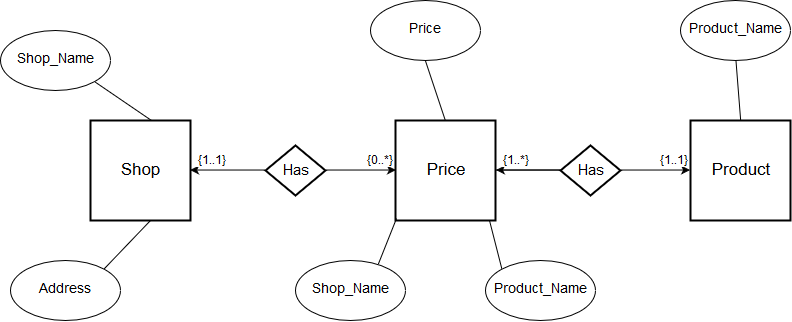
\includegraphics[width=\textwidth ,height=6cm]{ERD.png}
  \centering
  \caption{SRRec Entity-Relationship Diagram}
  \label{fig:Entity-Relationship Diagram}
\end{figure}

\begin{figure}[H]
  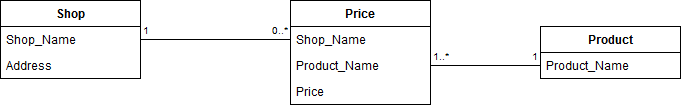
\includegraphics[width=\textwidth ,height=4cm]{ClassDiagram.png}
  \centering
  \caption{SRRec UML Class Diagram:association class as a full class(Price)}
  \label{fig:Class Diagram}
\end{figure}



\subsection{Data Flow Diagram(DFD)}
The process begins when the Shopper (user) requests for a recommended shopping route. The system will retrieve a list of product names from the Product datastore and display them for the user to select their required products. These selected products will be logged into the shopping list, which is stored temporarily on the web-application. When the user has completed their shopping list, the system will search for shops from the Shop datastore that sell the required products. These relevant shop addresses will then be parsed to the “Generate Shortest Path” function where the web-application will make use of Google Maps API (external tool) to map the recommended route and thus display it to the user.\\\\
Note: It is assumed that the user requires the route immediately after logging the products in the shopping list.\\

\begin{figure}[H]
  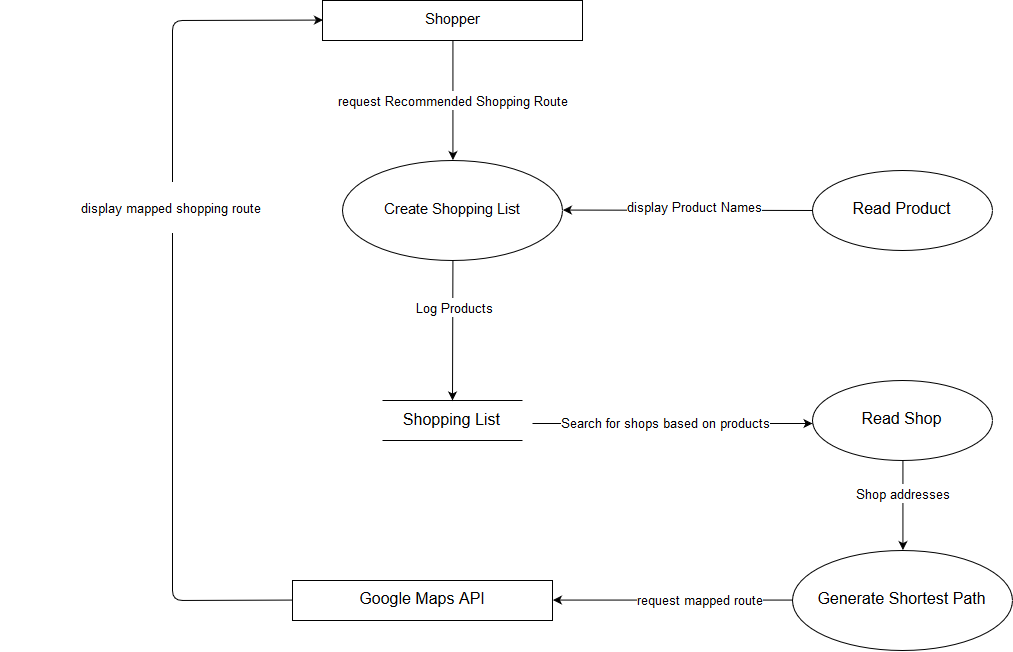
\includegraphics[width=\textwidth ,height=8cm]{DFD.png}
  \centering
  \caption{SRRec Data Flow Diagram}
  \label{fig:Data Flow Diagram}
\end{figure}

\subsection{Class-Responsibility-Collaborators (CRC) Cards}
We decided to make use of CRC cards, because they are helpful for early analysis in software development. These cards help identify/specify system and design components, quickly and informally.\\

\begin{figure}[H]
  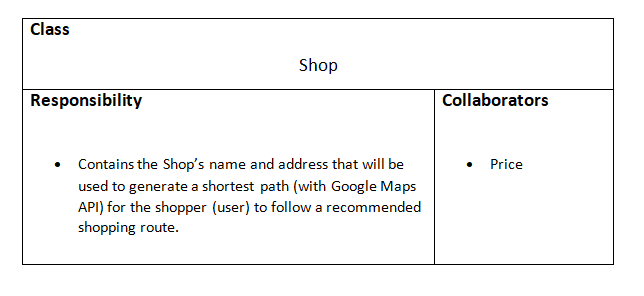
\includegraphics[width=\textwidth ,height=8cm]{ShopCRC.png}
  \centering
  \caption{SRRec Shop CRC}
  \label{fig:Shop CRC}
\end{figure}

\begin{figure}[H]
  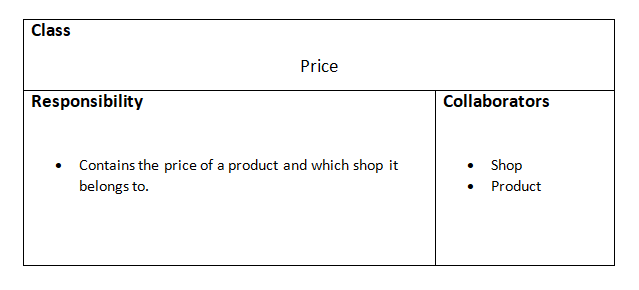
\includegraphics[width=\textwidth ,height=8cm]{PriceCRC.png}
  \centering
  \caption{SRRec Price CRC}
  \label{fig:Price CRC}
\end{figure}

\begin{figure}[H]
  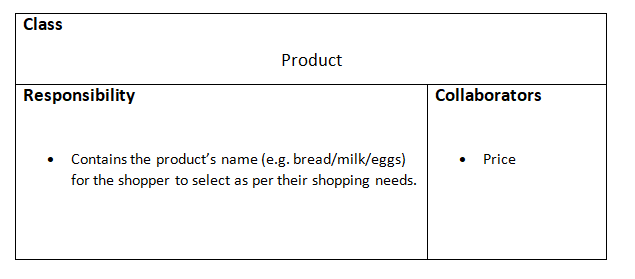
\includegraphics[width=\textwidth ,height=6cm]{ProductCRC.png}
  \centering
  \caption{SRRec Product CRC}
  \label{fig:Product CRC}
\end{figure}

\subsection{Sequence Diagram}
The SRRec sequence diagram follows the same logic process/flow as the data flow diagram (DFD).
\\
The Shopper (user) requests for a recommended shopping route. The process will then start and the system will request a list of product names from the Product datastore. These product names will be displayed for the user to select their required products. These selected products will be logged into the shopping list, which is stored temporarily on the web-application. When the user has completed their shopping list, the system will search for shops from the Shop datastore that sell the required products. These relevant shop addresses will then be parsed to the Google Maps API (external tool) in order to map the recommended route and thus display it to the user.
\\\\
Note: It is assumed that the user requires the route immediately after logging the products in the shopping list. The shopping list is cleared when the user closes the web-application, and will therefore be required to start a new shopping list the next time they request a recommended shopping route.\\

\begin{figure}[H]
  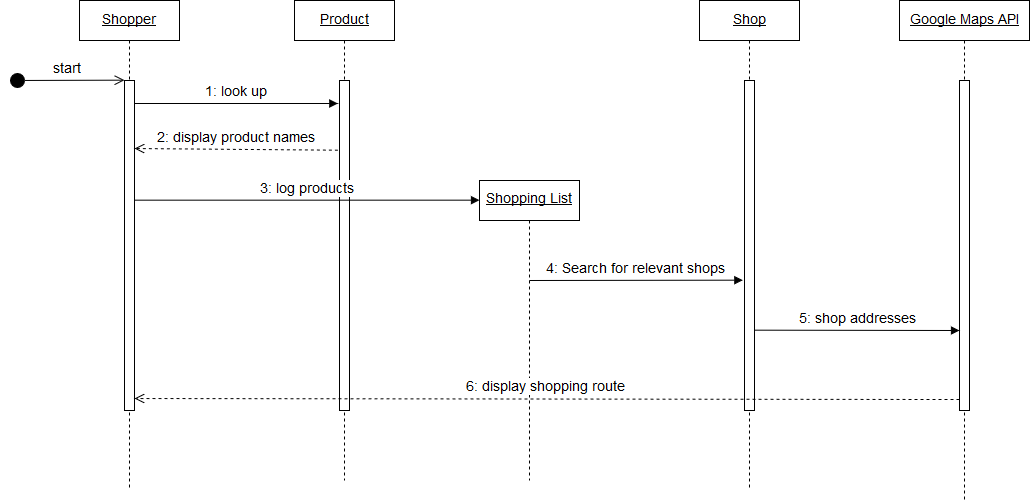
\includegraphics[width=\textwidth ,height=10cm]{SequenceDiagram.png}
  \centering
  \caption{SRRec Sequence Diagram}
  \label{fig:Sequence Diagram}
\end{figure}


\subsection{Use Case Diagram}
The use case diagram provides an overview of the set of use cases and the actors that interact with them.\\
Our system has four actors: The Shopper (user), Developer and two external actors, the Shop Outlet and Google Maps API.\\
Because our system makes use of Product and Price data that is retrieved from their respective Shop databases, the Shop Outlet is responsible for providing us with updated and correct data.\\
The Developer is responsible for the maintenance of the system’s functional processes as well as which Shops are added or removed from the system.\\
The Shopper (user) will view the products available when creating and logging their shopping list,and thus request a recommended shopping route/shortest path.\\
The external actor, Google Maps API, will be the external tool used to generate the shortest path by mapping the relevant shops and displaying the route to the user.\\

\begin{figure}[H]
  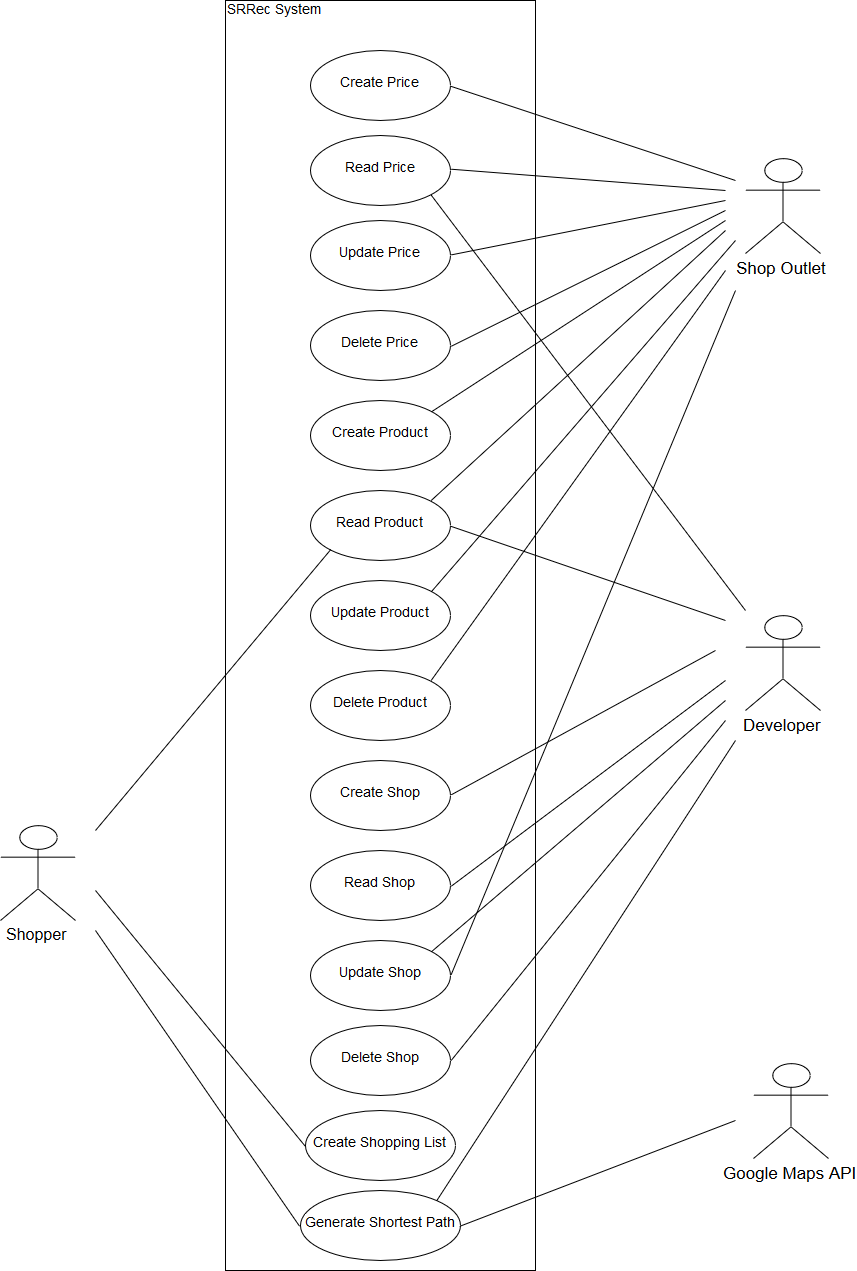
\includegraphics[width=\textwidth ,height=20cm]{UseCaseDiagram.png}
  \centering
  \caption{SRRec Use Case Diagram}
  \label{fig:Use Case Diagram}
\end{figure}


\section{Sprint Retrospective}
\subsection{Sprint 1: 24 Aug-31 Aug}
\underline{What did we do well?}
\begin{itemize}
\item Team was quick to identify the pros and cons of using different architectures
\item Each member researched their relevant architectures in great depth to ensure that the correct one was chosen for the problem 
\end{itemize}
\underline{What could we have done better?}
\begin{itemize}
\item Communication between team members needs to improve 
\item Spent less time of this sprint as too much time was allocated for research 
\end{itemize}
\underline{What should we start doing?}
\begin{itemize}
\item Make greater use of our KanBan scrum board to show the scrum master we are on schedule
\end{itemize}

\subsection{Sprint 2: 31 Aug-7 Sep}
underline{What did we do well?}
\begin{itemize}
\item Design was agreed upon quickly so as to avoid excess back and forth
\item Team members took upon the tasks they have strengths in
\item Use of the Scrum board was better
\end{itemize}
\underline{What could we have done better?}
\begin{itemize}
\item Drawing up designs took too much time
\item Daily stand-ups all started late
\item Communications in daily stand-ups needs to improve
\end{itemize}
\underline{What should we start doing?}
\begin{itemize}
\item Introduce a design standard through out the project
\item Make use of team Whatsapp group for Q\&A
\end{itemize}
\underline{What should we keep doing?}
\begin{itemize}
\item Assigning tasks on the scrum board to ourselves so members know who's working on what and how we're progressing 
\end{itemize}

\subsection{Sprint 3: 7 Sep-21 Sep}
\underline{What did we do well?}
\begin{itemize}
\item Tasked were assigned to members who wanted to work on those tasks and that played to their strengths
\item Communication on team Whatsapp group was greatly improved 
\item Daily stand-ups took place on time
\item Tasks were completed in a timeous manner
\end{itemize}
\underline{What could we have done better?}
\begin{itemize}
\item Backups of all code and data
\item Could have created our database in 3rd Normal Form rather than having to normalise it
\item Instituted a naming standard
\item Delegate tasks between the team better
\end{itemize}
\underline{What should we start doing?}
\begin{itemize}
\item Pushing code to GITHUB 
\item Implementing a naming standard
\item Do code reviews
\item Testing
\end{itemize}
\underline{What should we keep doing?}
\begin{itemize}
\item Keep assigning tasks on KanBan
\item Q\&A
\end{itemize}

\begin{figure}[H]
  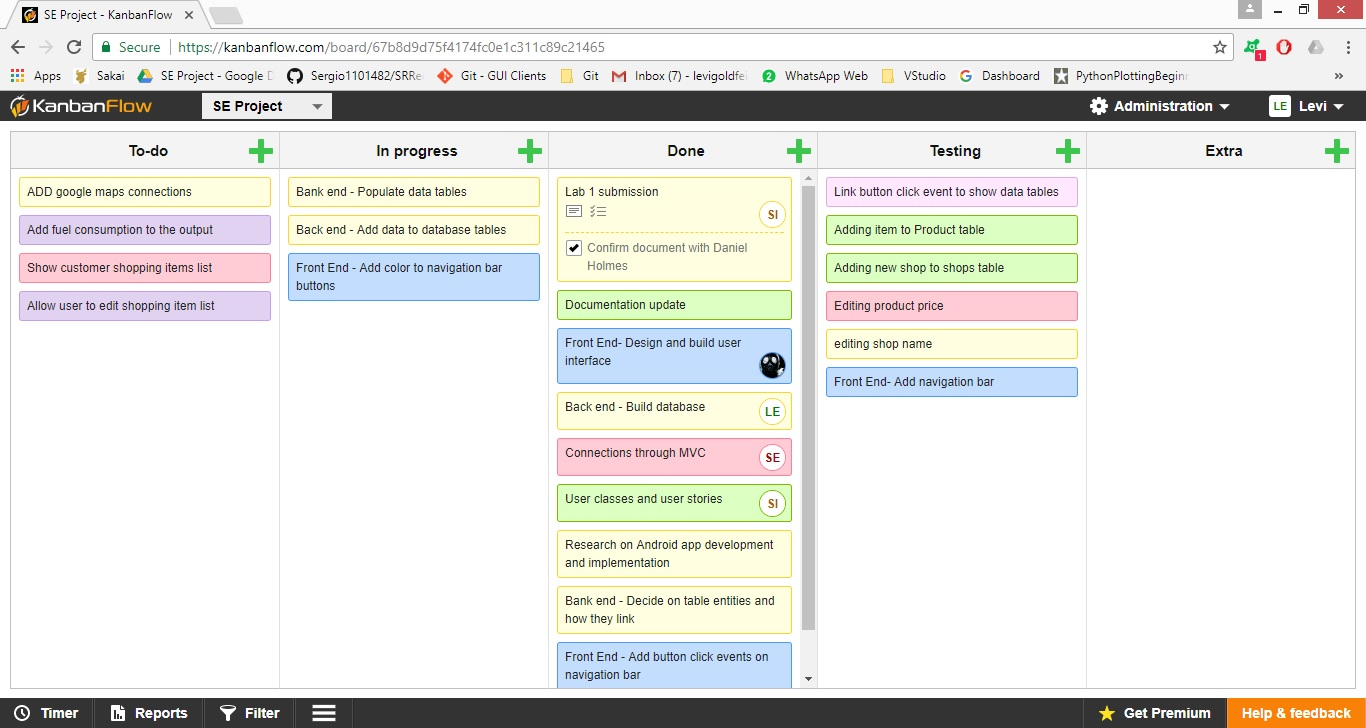
\includegraphics[width=15cm,height=10cm]{SprintBoard.jpg}
  \centering
  \caption{An example of our Sprint Board.}
%%%%  \label{fig:boat1}
\end{figure}

\section{How to compile code and start modules}
{\color{red} N.B The following software packages are required to compile and view the code
\begin{itemize}
\item Local DB
\item SQL Server
\item Visual Studio
\end{itemize}}
\hfill\\
After cloning the program from \url{https://github.com/Sergio1101482/SRRec.git}\\
\hfill
\textbf{Step 1:} Open Visual Studio\\
\textbf{Step 2:} Click \textbf{File}, then \textbf{Open}, then\textbf{Project/Solution}\\
\textbf{Step 3:} Navigate to \textbf{InterfaceSE} file (which will       be located in the cloned folder) and open it, then double click on \textbf{Interface.sln}\\
\textbf{Step 4:} Once loaded, click \textbf{Build} in the navigation bar, then click \textbf{Build Solution} and wait for the build to complete\\
\textbf{Step 5:} Run the program by clicking the \textbf{Run} button (the {\color{green} \textbf{GREEN}} play button in navigation bar)


\section{Testing}
\subsection{Back-End Testing}
\begin{center}
\begin{tabular}{| l | c |}
\hline  
\textbf{Back-end Tests} & \\ \hline
\textbf{TEST} & \textbf{PASS/FAIL} \\ \hline% heading
Retrieving entries from database & PASS\\ \hline
Shortest path calculation & PASS\\ \hline
Adding new product & PASS\\ \hline
Adding new shop & PASS\\ \hline
Delete product & PASS\\ \hline
Delete shop & PASS\\ \hline
Edit shop name & PASS\\ \hline
Edit price & PASS\\ \hline
Edit shop address & PASS\\ \hline
Edit product name & PASS\\ \hline
\end{tabular}
\end{center}

\subsection{Front-end Testing}
\begin{center}
\begin{tabular}{|l | c|}
\hline  
\textbf{Front-end Tests}&\\\hline
\textbf{TEST} & \textbf{PASS/FAIL} \\ \hline
Click button "Shopping Route Recommender"shows\\ "Shortest Path" button and "Lowest Cost" button  & PASS\\ \hline
Click "Shortest Path" button shows\\
table of products on screen & PASS\\ \hline
Click "Lowest Cost" shows \\"Functionality to come with update" message & PASS\\ \hline
Click on products on tables makes them grey out & PASS\\ \hline
Click on products on tables adds them to selected list & PASS\\ \hline
Click "Done" button displays shortest path on screen & PASS\\ \hline
Click "About Us" button shows\\"Description" and "Contact Us" buttons & PASS\\ \hline
Click "Description" button shows\\ company description on screen & PASS\\ \hline
Click "Contact Us" button shows\\ company contact information & PASS\\ \hline
Click "Help" button shows\\"FAQ" and "How to Use" buttons & PASS\\ \hline
Click "FAQ" button shows\\ all frequently asked questions & PASS\\ \hline
Click "How to Use" button show\\ How to make use of the application screen & PASS\\ \hline
Click "Settings" button shows\\ "Customise" and "Account Settings" buttons & PASS\\ \hline
Click "Customise" shows\\"Functionality to come with update" message & PASS\\ \hline
Click "Account Settings" shows\\"Functionality to come with update" message & PASS\\ \hline
\end{tabular}
\end{center}

\end{document}